\section{The \sysname Design}
\label{sec:system}
% Basic what it is
\sysname is a slim, batteryless, occupancy-monitoring sensor system mounted to the top of a doorframe.
It is powered by energy harvested from two arrays of indoor solar panels pointed at the floor.
The panels serve two roles: 1)~energy harvester and 2)~sensor.
These panels gather \textbf{energy} for computation, sensing, and signaling while also providing the \textbf{signal} that \sysname uses to detect when a person walks through the doorway in the form of variations in the harvested energy.
\sysname records the direction---entry or exit---of each doorway event and stores this information in non-volatile memory for later transmission.


\noindpar{Design Goals:} Unpredictable power supplies and human behaviors make designing an intermittently-powered occupancy sensor challenging.
We designed \sysname to meet the following design goals. 

%uncomment to save a few lines.
%\begin{enumerate}[wide, labelwidth=!, labelindent=0pt]
\begin{enumerate}
	\item \textbf{Availability:} Doorway events can occur at any time.
	While many intermittent sensors gather data opportunistically as energy is available, \sysname is designed to conserve its harvested energy so that it is available to detect ephemeral doorway events, whenever they occur.
	\item \textbf{Accurate direction:} In addition to detecting someone passing through the doorway, \sysname uses angled solar panels to accurately determine their direction.
	This plays a crucial role in inferring the occupancy of rooms and buildings.
	\item \textbf{Variable lighting conditions:} Indoor lighting conditions can change over time, due to human behavior and the relative movement of the sun.
	We have designed \sysname to work in a range of different lighting conditions by using detection circuits that respond to changes in light level, independent of the absolute amount of light, as well as tuning mechanisms built into the prototype.
	\item \textbf{Variable human characteristics:} An effective occupancy sensor should work well in spite of variations in clothing, hair, height, walking speed, and skin color. By focusing on changes in total reflected light, \sysname is robust to these human variations.
	\item \textbf{Form factor:} We want \sysname to be easy to deploy, to fit unobtrusively inside a door frame, and avoid contact with doors (on frames with doors).
	We could harvest more energy by wrapping \sysname around the doorframe, but the system would be more expensive, harder to deploy, and more likely to interfere with doors, while also changing the aesthetics of the doorway.
\end{enumerate}

\noindpar{What \sysname is not.}
We also want to be clear about what \sysname is \emph{not}.
\sysname is \emph{not} a security device.
\sysname helps building owners and managers understand how people move through buildings, but it is \emph{not} designed to thwart malicious behavior.
We can easily trick \sysname with a flashlight or reflective materials, and we can disable it completely by covering its solar panels or turning off the lights.
Users looking to prevent shenanigans or tomfoolery should use a different device.
Users looking for a long-lived, low-maintenance, best-effort batteryless occupancy sensor for monitoring normal behaviors should read on.

% fig refs
\noindpar{}
The \sysname hardware architecture, shown in \figref{fig:overview}, includes support for energy harvesting, event detection, computation, and communication.
% Intro the rest of the section
In this section, we describe these components and how they work together to meet \sysname's design goals.


\begin{figure}[t]
\centering
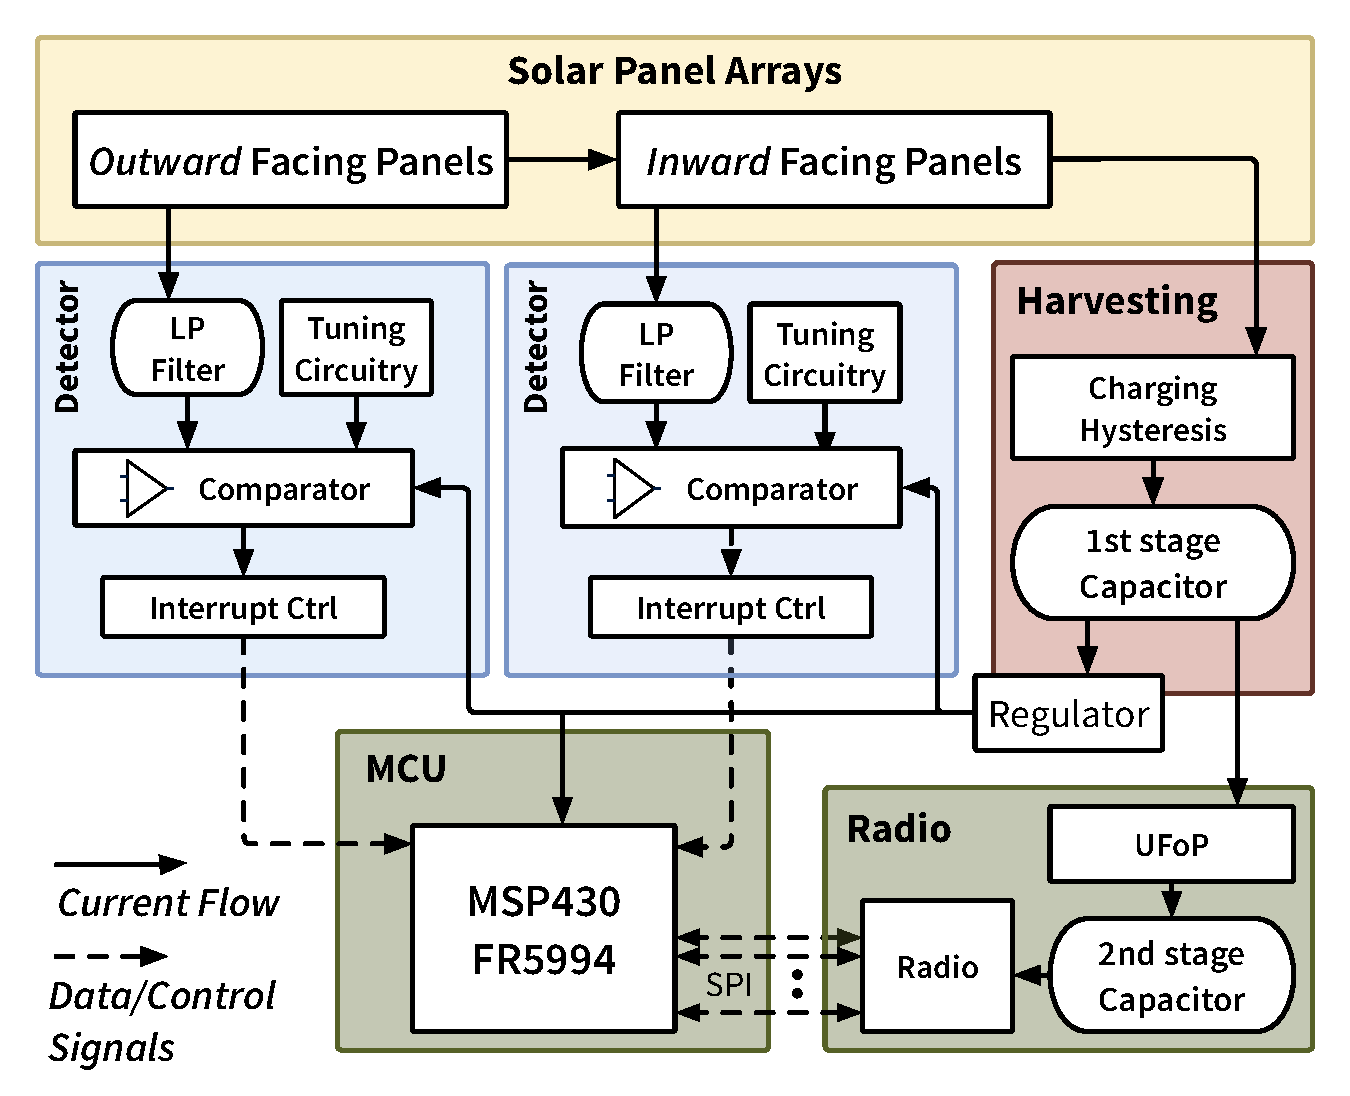
\includegraphics[width=0.55\columnwidth]{figs/overview.pdf}
\caption{The \sysname architecture overview. \sysname uses the energy and signals from two sets of solar panels to both power the sensor and detect people passing into and out of a doorway. Two detector circuits each monitor the solar panels sets mounted in series in the doorway. One detector monitors a set of similarly facing panels, while the other observes the combined signal from all of the panels. On detection, the detectors wake up the MCU to process, log, or communicate occupancy information.  \label{fig:overview}}
\end{figure}


\subsection{Energy Harvesting and Management}
\sysname takes advantage of the ubiquity of indoor light in homes and offices.
Solar panels are mounted to the top of the door frame, pointing down toward the floor---half tilted \ang{20} inward and half tilted \ang{20} outward.
Pointing the panels downward is not ideal for energy harvesting but effective for detecting doorway events and provides a slim, easy-to-deploy unobtrusive form factor.
Tilted panels help \sysname determine walking direction, since a person will affect one half of the panels before the other. 
%\fxnote{[Not sure if this needs to be reworded since half of the panels might not accurately represent what is going on here.  Maybe instead -- will trigger one of the detectors at varying times, or something like this.-NT  The statement is true, and clarified in the next paragraph. This is fine. -JMS]}

To maximize energy harvesting, we connect the two sets of solar panels---the inward-facing set and the outward-facing set---in series.  
A series configuration conveniently combines the two panel sets into a single power source that can be used without adding boost regulators or other power conditioning circuitry.
This configuration makes it more difficult to analyze the two signals independently since they lack a common ground\footnote{For a series connection, we connect the positive terminal of the first panel set to the negative terminal of the second.}.
Instead, we measure the voltage of the outward-facing set alone, and the combination of the two sets.
We could compute the inward panels' voltage by subtracting the two; however, we have found that we can skip this step and just compare the two measurements directly, as shown in \figref{fig:traces}, to determine walking direction.


\sysname uses federated energy storage~\cite{jhester:ufop:sensys} to power its microcontroller and peripherals.
Harvested solar energy is fed into a common first-stage storage capacitor and then automatically federated to its one peripheral---a Texas Instruments CC1101 radio.
Federating energy allows us to start detecting and processing events while saving up energy for more energy-expensive radio transmissions.
It also improves harvesting efficiency and reduces the risk that the microcontroller will lose power due to a radio transmission.

\begin{figure*}[t]
	\centering
	\begin{subfigure}[b]{0.45\textwidth}
		\centering
		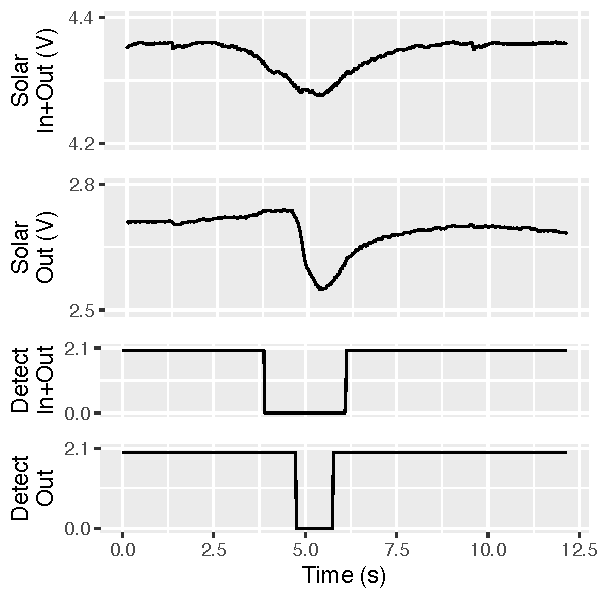
\includegraphics[width=0.8\columnwidth]{figs/tracesin.pdf}
		\caption{Walking in.}
		\label{fig:tracesin}
	\end{subfigure}%
	%
	\begin{subfigure}[b]{0.45\textwidth}
		\centering
		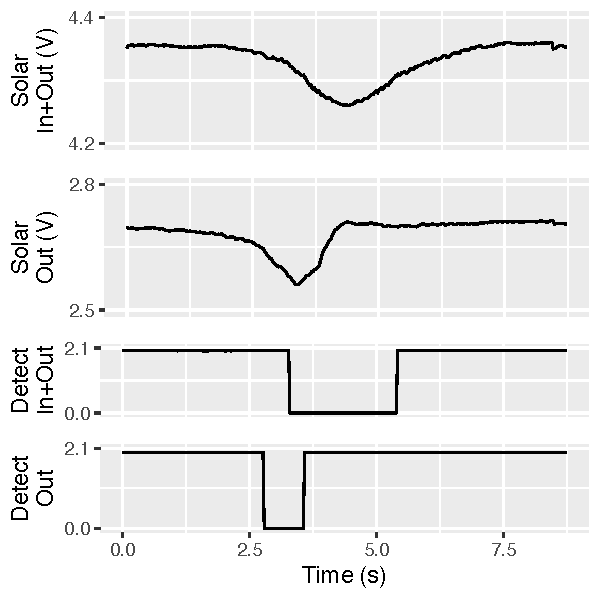
\includegraphics[width=0.8\columnwidth]{figs/tracesout.pdf}
		\caption{Walking out.}
		\label{fig:tracesout}
	\end{subfigure}
	\caption{These traces show example solar panel voltages and detector outputs over time when a person walks through a \sysname-enabled doorway. The top traces show how the solar panel's voltages are deformed during the doorway event. The detector triggers are used to wake up the microcontroller and detect events and their direction. The angling of the panels cause the inward facing and outward facing detectors to trigger at different times depending on the direction the person is walking.\label{fig:traces}}
\end{figure*}

\subsection{Detection}
\label{sec:detection}



%\fxnote{[It would be nice to do this data driven off some traces gathered. Simulate, essentially, just by doing some light math. So how do we capture the waveforms when we trigger the wakeup? - JDH]}

%what happens when a person walks through.
When someone walks under \sysname, they block some of the reflected light hitting the solar panels.
In \figref{fig:traces}, the solar traces on top show how solar panel voltage changes during a doorway event.

In order to detect a doorway event, we could use an ADC to continuously measure the solar panel voltage over time and analyze those readings to detect the presence and, more importantly, direction of motion.
Voltage levels and waveform shapes vary with lighting conditions, especially when one side of the doorway has more natural light.
This approach would mean more complicated signal analysis and much higher energy consumption.
Instead, \sysname uses a \textbf{detection circuit} that wakes up the microcontroller when it detects a significant change in the solar panel voltage over a short period of time.
This circuit consists of a passive first-order capacitive filter connected to a nano-power comparator---producing a square wave that transitions when the voltage increases or decreases faster than a set rate.
These transitions trigger interrupts that help \sysname detect when someone is passing through the doorway.

In order to determine movement direction, we use two detector circuits: one that detects change on the outward-facing panels and another that detects change on the combined inward- and outward-facing panels.
When someone walks through the doorway, the detectors trigger at different times, depending on the walking direction, as shown in \figref{fig:traces}.
\sysname compares the timing of these detector interrupts to distinguish incoming and outgoing events.


\noindpar{Removing light flicker.}
Many fluorescent indoor lights flicker at \SI{60}{\hertz} or higher---a much higher frequency than the events \sysname detects.
If not filtered out, fluctuations can confuse the detection circuit and produce false positive results.
We add a low-pass filter to remove noise above \SI{10}{\hertz} from the solar panel signal.

\noindpar{Isolating harvesting from sensing.}
If connected directly, \sysname's harvesting and event detection circuits can potentially conflict in two important ways.
First, the harvesting circuit stores harvested energy in a \SI{100}{\micro\farad} capacitor---a size that ensures that \sysname can store enough energy for short-term tasks and dampens the low-frequency voltage fluctuations that we need in order to detect doorway events.
Second, short-term power spikes from interrupt service routines and other computation cause high-frequency dips in the solar voltage, which can confuse the detection circuits.
We address both of these challenges by adding an additional low-pass filter between the detection and harvesting circuits. This isolates the solar panel from the load, and allows the solar panel voltage (after the initial flicker filter) to fluctuate over a wider range in response to doorway events with less interference from the storage capacitor, the microcontroller power draw, and the detector circuit power draw. 

\noindpar{Detection algorithm:}
\sysname's software works as shown in \figref{fig:software}. 
During normal operation, when no doorway events are detected, \sysname's MCU remains in a sleep mode, only waking up to report heartbeats after two minutes of inactivity.
While in sleep mode, the MCU only wakes up in two cases: 1)~when its inter-event timer fires (this timer measures the time that has passed since the last reported event) and 2)~when activity near the sensor triggers the detector circuits.
A detector transition from a high state to a low state---due to a drop in harvested solar energy caused by a person walking through the doorway---will wake up the system to process an event.
This initial wake-up marks the start of an event.
The MCU records when the interrupt occurred, starts an event timer~(6 seconds), and goes back into sleep mode.
During the \SI{6}{\second} event, the MCU will wake up each time the detectors transition (from HIGH to LOW and vice versa) to record the length of time between each transition.
A person may block light in many ways, and so multiple interrupts may fire during a single doorway event.
When the event timer fires (after \SI{6}{\second}), the event is considered finished and event classification and recording begins.

\begin{figure}[t]
\centering
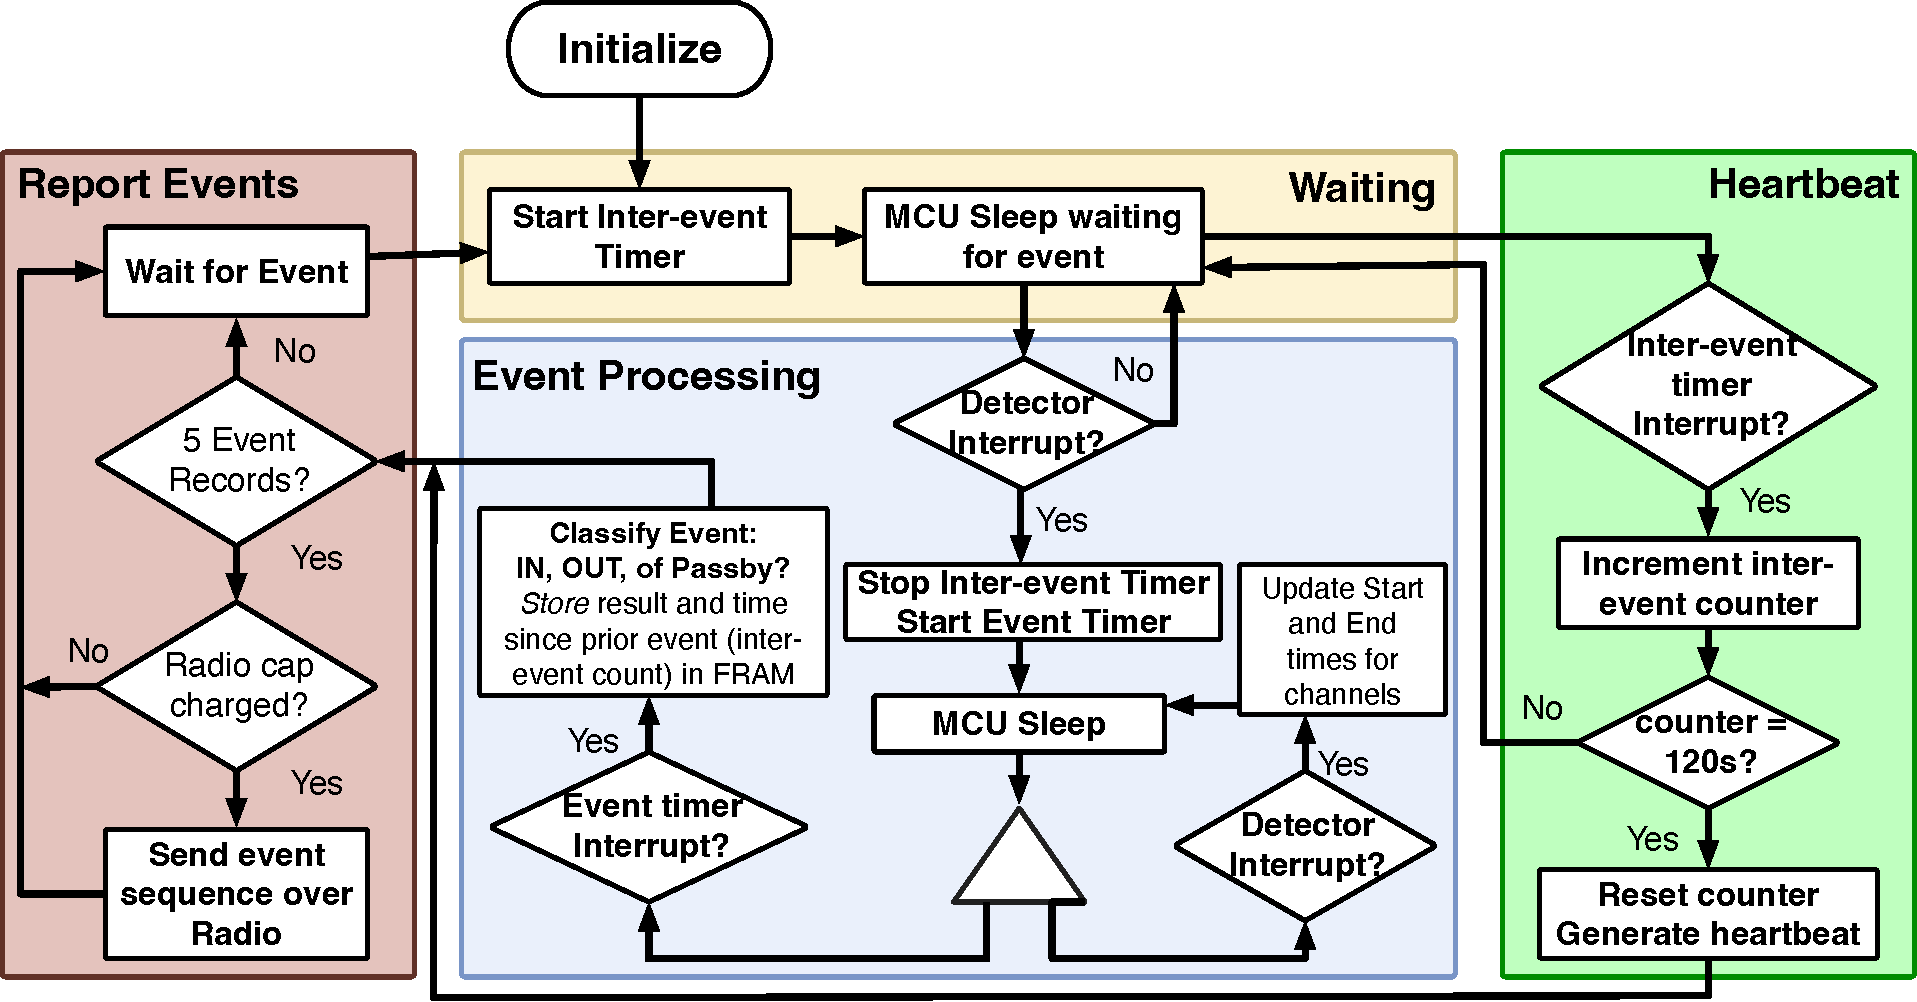
\includegraphics[width=0.75\columnwidth]{figs/software_update.pdf}
\caption{The \sysname detection algorithm and system decision flowchart. The algorithm is composed of four parts that handle reporting doorway events, processing detected events, processing time between events and heartbeats, and idle waiting. \label{fig:software}}
\end{figure}


Times are recorded for the first falling edge interrupt (start time) and the last recorded rising edge (end time) for both solar panel sets of inward and outward facing panels.
When the event timer fires, the system has recorded both solar panel sets' start and end times, which are the features used to classify the event.
%For initial testing, we simply compare these times to determine the direction of the event (entry or exit), and the \sysname stores the detected event in non-volatile memory.
For training, we collected features from 332 controlled events from two different people at three different locations, a lab, an office, and a hallway.
Using this data, we trained a 4-layer decision tree that classifies events as INs, OUTs, and PASS-BYs (when a person passes within a few feet of the sensor, but not under it.)
When locations had a door, the door remained open for the collection.  %
% These events allowed us to not only train the system on standard ins and outs, but also on variations of passing by a doorway (a foot away to a couple of feet away on both sides of the system) which could trigger false ins and outs in the system.  A 4-layer decision tree was trained on 70\% of the events and tested on the remaining ones - achieving a 93.25\%-94.38\% accuracy.  
The trained decision tree is then used on \sysname to classify observed events during deployments.  


Between events, \sysname uses an inter-event timer to estimate time between events.  
When the next event is detected, the inter-event timer is stopped and then the event timer is started for processing the event interrupts during the event window.
A heartbeat record is generated when the time since the last event passes 120 seconds and is added to packet information to be sent with other records to the basestation. 
Once the event is processed and classified or heartbeat is generated, it is recorded in non-volatile memory along with the estimated time that has past since the last event or heartbeat record.  
The inter-event timer is then reset and the cycle continues.


\subsection{Communication and Infrastructure}
\sysname's collected data are stored in non-volatile memory until the system has saved up enough energy to transmit.
To reduce transmission cost, we summarize the last~5 recently-detected event records, sending the sequence of events in order of when they were recorded with the estimated time since the last event that was seen and the classification of that event as an in, out, passby, or heartbeat when 2 minutes of inactivity is recorded.
We compute a CRC over each sequence summary and send the prior two sequence summaries in each packet to reduce the risk of losing information due to corrupted or missing packets and increase the likelihood that a basestation will receive the data. 
If the radio's capacitor isn't sufficiently charged, \sysname will sleep and try again when the next event occurs.
This pattern continues throughout the system's operational lifetime.

%\subsection{Adaptation}
%\fxnote{[Remove this - JDH]}

%\sysname dynamically changes task sets depending on energy availability - attempting to assign higher energy tasks when energy is more available in the environment and assigning lower energy tasks assigned when energy is scarce in the environment. \fxnote{[Does not do this, need to remove - JDH]}
%These tasks correspond to different tiers of quality of service (QoS) of the application, with the highest level providing real time event marking on door traffic coupled with person identification using heights, hair color, and wardrobe. \fxnote{[Does not do this either, need to remove - JDH]}
%The lowest QoS tier corresponds to only logging entry and exit, and sending a summary of the data opportunistically over the radio. \fxnote{[Does not do this either! Put in future work- JDH]}
